\documentclass{standalone}

\usepackage{standalone}
\usepackage{tikz}
\usetikzlibrary{er,positioning, calc}

\begin{document}

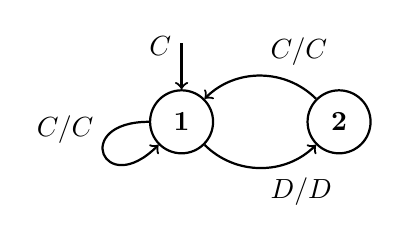
\begin{tikzpicture}
	\tikzstyle{state}=[minimum width=0.8cm, font=\boldmath];

   \node[circle, draw=black, thick] (1) at (5, 0) [state]    {$1$};
   \node[circle, draw=black, thick] (2) at (7, 0) [state]    {$2$};
   \coordinate (s) at (5, 1);
   \draw (s) edge[out=-90, in=90, ->, thick] node [above left] {$C$} (1);
   \draw (1) edge[out=180, in=-135, ->, thick, loop, looseness=8] node [above left] {$C/C$} (1);
   \draw (1) edge[out=-45, in=-135, ->, thick] node [below right] {$D/D$} (2);
   \draw (2) edge[out=135, in=45, ->, thick] node [above right] {$C/C$} (1);
   

\end{tikzpicture}
\end{document}